\section {Methods}


\begin{figure*}[h]
\caption{
Universal Schema jointly embeds KB and textual relations from Spanish and English, learning dense representations for entity pairs and relations using matrix factorization. Cells with a 1 indicate triples observed during training (left). The bold score represents a test-time prediction by the model (right). Using transitivity through KB/English overlap and English/Spanish overlap, our model can predict that a text pattern in Spanish evidences a KB relation despite no overlap between Spanish/KB entity pairs.
At train time we use BPR loss to maximize the inner product of entity pairs with KB relations and text patterns encoded using a bidirectional LSTM. At test time we score compatibility between embedded KB relations and encoded textual patterns using cosine similarity. In our Spanish model we treat embeddings for a small set of English/Spanish translation pairs as a single word, e.g. casado and married.
\label{fig:model}}
  \hspace{-.75cm}%
\begin{subfigure}{.7\textwidth}
    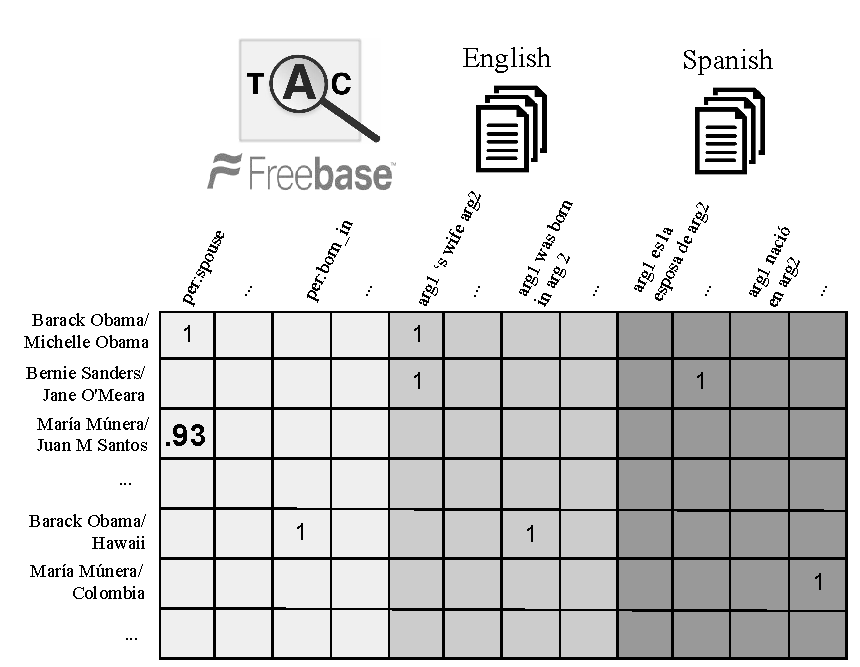
\includegraphics[scale=.7]{matrix}
\end{subfigure}%
  \hspace{-.75cm}%
\begin{subfigure}{.4\textwidth}
  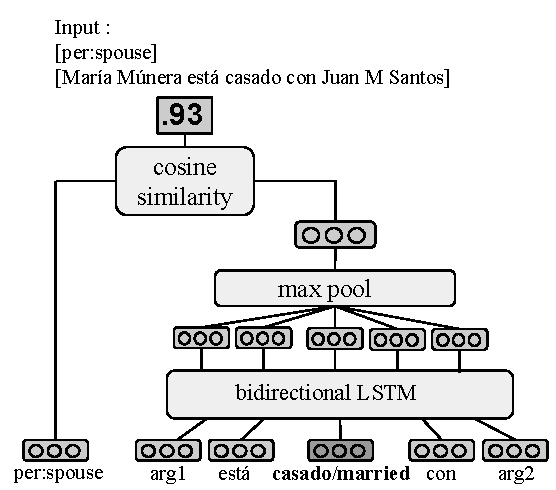
\includegraphics[scale=.8]{model-score}
\end{subfigure}
\end{figure*}

%\section{Training a Sentence Classifier without Alignment \label{sec:uschema}}
\subsection{Universal Schema as Sentence Classifier \label{sec:uschema}}
%\todo{Reviewer 2: Sec. 3 mainly talks about prediction (matching a text pattern with a KB relation, instead of direct prediction based on entity pairs), but the title is training a sentence classifier}
Similar to many link prediction approaches,~\citep{limin} perform transductive learning, where a model is learned jointly over train and test data. Predictions are made by using the model to identify edges that were unobserved in the test data but likely to be true. The approach is vulnerable to the \emph{cold start} problem in collaborative filtering~\citep{schein2002methods}: it is unclear how to form predictions for unseen entity pairs, without re-factorizing the entire matrix or applying heuristics.

In response, this paper re-purposes USchema as a means to train a sentence-level relation classifier, like those in Section~\ref{seq:dist}. This allows us to avoid errors from aligning distant supervision to the corpus, but is more deployable for real world applications. It also provides opportunities in Section~\ref{sec:multilingual} to improve multilingual AKBC.

We produce predictions using a very simple approach: (1) scan the corpus and extract a large quantity of triplets $(s,r_{\text{text}},o)$, where $r_{\text{text}}$ is an OpenIE pattern. For each triplet, if the similarity between the embedding of $r_{\text{text}}$ and the embedding of a target relation $r_{\text{schema}}$ is above some threshold, we predict the triplet $(s,r_{\text{schema}},o)$, and its provenance is the input sentence containing $(s,r_{\text{text}},o)$. We refer to this technique as~\textit{pattern scoring}. In our experiments, we use the cosine distance between the vectors (Figure \ref{fig:model}).

%% APPENDIX %% In Section~\ref{app:cosine}, we discuss details for how to make this distance well-defined.


\subsection{Using a Compositional Sentence Encoder to Predict Unseen Text Patterns \label{sec:encoder}}
%\todo{Reviewer 2: Sec. 4 explains how to encode textual patterns with some neural network architectures, and this is clearly used in both training and testing and the title is predictions for unseen text patterns}
The pattern scoring approach is subject to an additional cold start problem: input data may contain patterns unseen in training. This section describes a method for using USchema to train a relation classifier that can take arbitrary context tokens (Section~\ref{sec:openIE}) as input.

Fortunately, the cold start problem for context tokens is more benign than that of entities since we can exploit statistical regularities of text: similar sequences of context tokens should be embedded similarly. Therefore, following \citet{toutanova2015representing}, we  embed raw context tokens compositionally using a deep architecture. Unlike~\citet{limin}, this requires no manual rules to map text to OpenIE patterns and can embed any possible input string. The modified USchema likelihood is:
\begin{equation}
\Prob \left((s,r,o)\right) = \sigma\left( u_{s,o}^\top \text{Encoder}(r) \right).
\end{equation}
Here, if $r$ is raw text, then $\text{Encoder}(r)$ is parameterized by a deep architecture. If $r$ is from the target schema, $\text{Encoder}(r)$ is a produced by a lookup table (as in traditional USchema). Though such an encoder increases the computational cost of test-time prediction over straightforward pattern matching, evaluating a deep architecture can be done in large batches in parallel on a GPU.

Both convolutional networks (CNNs) and recurrent networks (RNNs) are reasonable encoder architectures, and we consider both in our experiments. CNNs have been useful in a variety of NLP applications~\citep{collobert2011natural,KalchbrennerACL2014,kim2014convolutional}. Unlike~\citet{toutanova2015representing}, we also consider RNNs, specifically Long-Short Term Memory Networks (LSTMs)~\citep{lstm}. LSTMs have proven successful in a variety of tasks requiring encoding sentences as vectors~\citep{rnnmt,rnnparse}. In our experiments, LSTMs outperform CNNs.

There are two key differences between our sentence encoder and that of~\citet{toutanova2015representing}.  First, we use the encoder at test time, since we process the context tokens for held-out data. On the other hand,~\citet{toutanova2015representing} adopt the transductive approach where the encoder is only used to help train better representations for the relations in the target schema; it is ignored when forming predictions.  Second, we apply the encoder to the raw text between entities, while~\citet{toutanova2015representing} first perform syntactic dependency parsing on the data and then apply an encoder to the path between the two entities in the parse tree. We avoid parsing, since we seek to perform multilingual AKBC, and many languages lack linguistic resources such as treebanks. Even parsing non-newswire English text, such as tweets, is extremely challenging. %Using the raw data, however, is  challenging since the raw text between two entities may be quite long. On the other hand, training a deep architecture end-to-end to identify the relevant text between entities is more practical for a variety of applications. \todo{pointer to experiments discussing parsed vs. unparsed data}


\subsection{Modeling Frequent Text Patterns}
\label{sec:non-comp}

Despite the coverage advantages of using a deep sentence encoder, separately embedding each OpenIE pattern, as in~\citet{limin}, has key advantages. In practice, we have found that many high-precision patterns occur quite frequently. For these, there is sufficient data to model them with independent embeddings per pattern, which imposes minimal inductive bias on the relationship between patterns. Furthermore, some discriminative phrases are idiomatic, i.e.. their meaning is not constructed compositionally from their constituents. For these, a sentence encoder may be inappropriate.
%using a sentence encoder induces shared structure across different patterns' representations.

Therefore, pattern embeddings and deep token-based encoders have very different strengths and weaknesses. One values specificity, and models the head of the text distribution well, while the other has high coverage and captures the tail. In experimental results, we demonstrate that an ensemble of both models performs substantially better than either in isolation.

%\begin{table}[h!]
%\begin{center}
%\caption{Examples of compositional vs. idiomatic text patterns for relation extraction.\label{tab:patterns2}}
%\begin{tabular}{| p{0.18\textwidth} | p{0.76\textwidth} | }
% \hline
% % who worked face to face with
% % a
% % started out as a
% % Toby Keith hit an emotional note with a performance of
% % , was convicted of all five counts against him , the most serious of them
%\multirow{3}{*}{compositional} & \argOne will be cremated on Friday just outside the city of \argTwo\\ %\cline{2-2}
%& \argOne has pleaded not guilty to charges of \argTwo \\ %\cline{2-2}
%& \argOne was convicted of all five counts against him, including \argTwo \\ %\cline{2-2}
%\hline
%\multirow{3}{*}{idiomatic} & \argOne , aka \argTwo \\ %\cline{2-2}
%& \argOne hit the field in \argTwo \\ %\cline{2-2}
%& \argOne didn't relish the idea of pulling the managerial rug out from under \argTwo \\
%\hline
%\end{tabular}
%\end{center}
%\end{table}


\subsection{Multilingual Relation Extraction with Zero Annotation \label{sec:multilingual}}

The models described in previous two sections provide broad-coverage relation extraction that can generalize to all possible input entities and text patterns, while avoiding error-prone alignment of distant supervision to a corpus. Next, we describe techniques for an even more challenging generalization task: relation classification for input sentences in completely different languages.

Training a sentence-level relation classifier, either using the alignment-based techniques of Section~\ref{seq:dist}, or the alignment-free method of Section~\ref{sec:uschema}, requires an available KB of seed facts that have supporting evidence in the corpus.  Unfortunately, available KBs have low overlap with corpora in many languages, since KBs have cultural and geographical biases. In response, we perform multilingual relation extraction by jointly modeling a high-resource language, such as English, and an alternative language with no KB annotation. This approach provides transfer learning of a predictive model to the alternative language, and generalizes naturally to modeling more languages.


Extending the training technique of Section~\ref{sec:uschema} to corpora in multiple languages can be achieved by factorizing a matrix that mixes data from a KB and from the two corpora. In Figure~\ref{tab:multilingual-corpora} we split the entities of a multilingual training corpus into sets depending on whether they have annotation in a KB and what corpora they appear in. We can perform transfer learning of a relation extractor to the low-resource language if there are entity pairs occurring in the two corpora, even if there is no KB annotation for these pairs. Note that we do not use the entity pair embeddings at test time: They are used only to bridge the languages during training. To form predictions in the low-resource language, we can simply apply the pattern scoring approach of Section~\ref{sec:uschema}.

In Section~\ref{sec:results}, we demonstrate that jointly learning models for English and Spanish, with no annotation for the Spanish data, provides fairly accurate Spanish AKBC, and even improves the performance of the English model. Note that we are not performing \textit{zero-shot} learning of a Spanish model~\citep{zeroshot}. The relations in the target schema are language-independent concepts, and we have supervision for these in English.



\subsection{Tied Sentence Encoders \label{sec:tie-words}}
The sentence encoder approach of Section~\ref{sec:encoder} is complementary to our multilingual modeling technique: we simply use a separate encoder for each language.  This approach is sub-optimal, however, because each sentence encoder will have a separate matrix of word embeddings for its vocabulary, despite the fact that there may be considerable shared structure between the languages. In response, we propose a straightforward method for tying the parameters of the sentence encoders across languages.

Drawing on the dictionary-based techniques described in Section \ref{sec:background-multilingual}, we first obtain a list of word-word translation pairs between the languages using a translation dictionary. The first layer of our deep text encoder consists of a word embedding lookup table. For the aligned word types, we use a single cross-lingual embedding.
%% APPENDIX %% Details of our approach are described in Section~\ref{sec:word-tying}.


